\documentclass{standalone}
\usepackage{tikz}
\usetikzlibrary{patterns, positioning}

\begin{document}
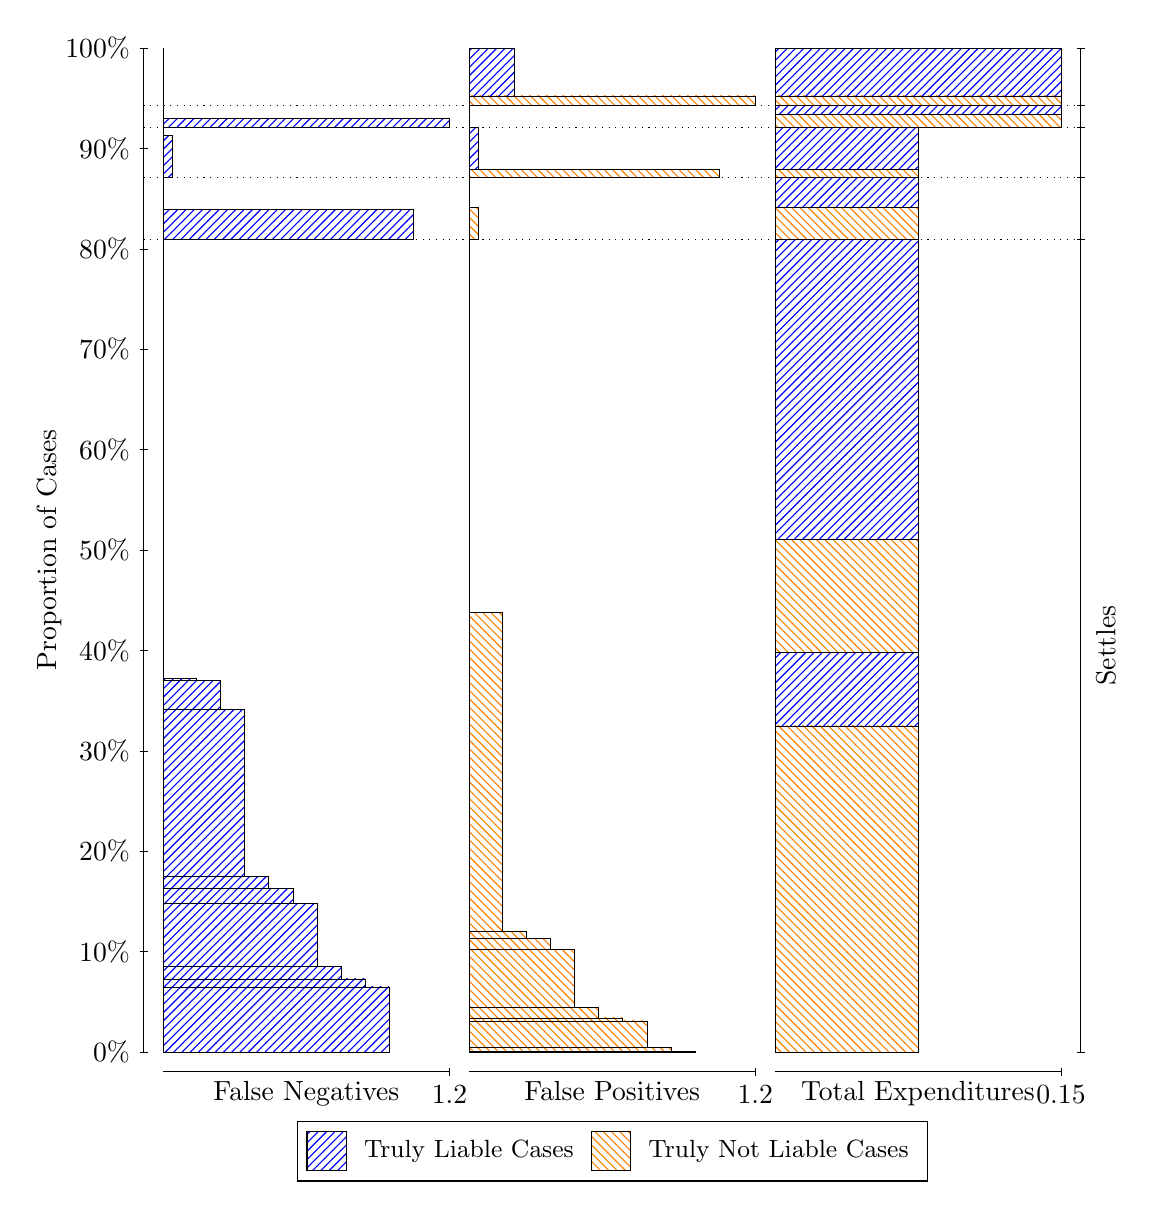
\begin{tikzpicture}
\draw[black, very thin] (1.5,1.75) -- (1.5,14.5);
\node[rotate=90, anchor=center] at (0.3, 8.125) {Proportion of Cases};
\draw[black, very thin] (1.45,1.75) -- (1.55,1.75);
\node[anchor=east] at (1.45, 1.75) {0\%};
\draw[black, very thin] (1.45,3.025) -- (1.55,3.025);
\node[anchor=east] at (1.45, 3.025) {10\%};
\draw[black, very thin] (1.45,4.3) -- (1.55,4.3);
\node[anchor=east] at (1.45, 4.3) {20\%};
\draw[black, very thin] (1.45,5.575) -- (1.55,5.575);
\node[anchor=east] at (1.45, 5.575) {30\%};
\draw[black, very thin] (1.45,6.85) -- (1.55,6.85);
\node[anchor=east] at (1.45, 6.85) {40\%};
\draw[black, very thin] (1.45,8.125) -- (1.55,8.125);
\node[anchor=east] at (1.45, 8.125) {50\%};
\draw[black, very thin] (1.45,9.4) -- (1.55,9.4);
\node[anchor=east] at (1.45, 9.4) {60\%};
\draw[black, very thin] (1.45,10.675) -- (1.55,10.675);
\node[anchor=east] at (1.45, 10.675) {70\%};
\draw[black, very thin] (1.45,11.95) -- (1.55,11.95);
\node[anchor=east] at (1.45, 11.95) {80\%};
\draw[black, very thin] (1.45,13.225) -- (1.55,13.225);
\node[anchor=east] at (1.45, 13.225) {90\%};
\draw[black, very thin] (1.45,14.5) -- (1.55,14.5);
\node[anchor=east] at (1.45, 14.5) {100\%};

\draw[black, very thin] (13.4,1.75) -- (13.4,14.5);
\draw[black, very thin] (13.35,1.75) -- (13.45,1.75);
\node[anchor=west] at (13.35, 1.75) {};
\draw[black, very thin] (13.35,12.074) -- (13.45,12.074);
\node[anchor=west] at (13.35, 12.074) {};
\draw[black, very thin] (13.35,12.858) -- (13.45,12.858);
\node[anchor=west] at (13.35, 12.858) {};
\draw[black, very thin] (13.35,13.49) -- (13.45,13.49);
\node[anchor=west] at (13.35, 13.49) {};
\draw[black, very thin] (13.35,13.773) -- (13.45,13.773);
\node[anchor=west] at (13.35, 13.773) {};
\draw[black, very thin] (13.35,14.5) -- (13.45,14.5);
\node[anchor=west] at (13.35, 14.5) {};

\draw[black, very thin, pattern color=blue, pattern=north east lines] (1.75,1.75) rectangle (4.6184,2.5778);
\draw[black, very thin, pattern color=blue, pattern=north east lines] (1.75,2.5778) rectangle (4.3125,2.6782);
\draw[black, very thin, pattern color=blue, pattern=north east lines] (1.75,2.6782) rectangle (4.0065,2.8343);
\draw[black, very thin, pattern color=blue, pattern=north east lines] (1.75,2.8343) rectangle (3.7005,3.6367);
\draw[black, very thin, pattern color=blue, pattern=north east lines] (1.75,3.6367) rectangle (3.3946,3.8294);
\draw[black, very thin, pattern color=blue, pattern=north east lines] (1.75,3.8294) rectangle (3.0886,3.9771);
\draw[black, very thin, pattern color=blue, pattern=north east lines] (1.75,3.9771) rectangle (2.7826,6.096);
\draw[black, very thin, pattern color=blue, pattern=north east lines] (1.75,6.096) rectangle (2.4767,6.4664);
\draw[black, very thin, pattern color=blue, pattern=north east lines] (1.75,6.4664) rectangle (2.1707,6.4907);
\draw[black, very thin, pattern color=orange, pattern=north west lines] (1.75,6.4907) rectangle (1.75,12.074);
\draw[black, very thin, pattern color=blue, pattern=north east lines] (1.75,12.074) rectangle (4.9244,12.454);
\draw[black, very thin, pattern color=orange, pattern=north west lines] (1.75,12.454) rectangle (1.75,12.858);
\draw[black, very thin, pattern color=blue, pattern=north east lines] (1.75,12.858) rectangle (1.8647,13.388);
\draw[black, very thin, pattern color=orange, pattern=north west lines] (1.75,13.388) rectangle (1.75,13.49);
\draw[black, very thin, pattern color=blue, pattern=north east lines] (1.75,13.49) rectangle (5.3833,13.607);
\draw[black, very thin, pattern color=orange, pattern=north west lines] (1.75,13.607) rectangle (1.75,13.773);
\draw[black, very thin, pattern color=orange, pattern=north west lines] (1.75,13.773) rectangle (1.75,13.892);
\draw[black, very thin, pattern color=blue, pattern=north east lines] (1.75,13.892) rectangle (1.75,14.5);
\draw[black, very thin, pattern color=orange, pattern=north west lines] (5.6333,1.75) rectangle (8.5018,1.7553);
\draw[black, very thin, pattern color=orange, pattern=north west lines] (5.6333,1.7553) rectangle (8.1958,1.8103);
\draw[black, very thin, pattern color=orange, pattern=north west lines] (5.6333,1.8103) rectangle (7.8898,2.1461);
\draw[black, very thin, pattern color=orange, pattern=north west lines] (5.6333,2.1461) rectangle (7.5839,2.1826);
\draw[black, very thin, pattern color=orange, pattern=north west lines] (5.6333,2.1826) rectangle (7.2779,2.3161);
\draw[black, very thin, pattern color=orange, pattern=north west lines] (5.6333,2.3161) rectangle (6.9719,2.3197);
\draw[black, very thin, pattern color=orange, pattern=north west lines] (5.6333,2.3197) rectangle (6.9719,3.0518);
\draw[black, very thin, pattern color=orange, pattern=north west lines] (5.6333,3.0518) rectangle (6.666,3.1918);
\draw[black, very thin, pattern color=orange, pattern=north west lines] (5.6333,3.1918) rectangle (6.36,3.2838);
\draw[black, very thin, pattern color=orange, pattern=north west lines] (5.6333,3.2838) rectangle (6.054,7.3335);
\draw[black, very thin, pattern color=blue, pattern=north east lines] (5.6333,7.3335) rectangle (5.6333,12.074);
\draw[black, very thin, pattern color=orange, pattern=north west lines] (5.6333,12.074) rectangle (5.7481,12.478);
\draw[black, very thin, pattern color=blue, pattern=north east lines] (5.6333,12.478) rectangle (5.6333,12.858);
\draw[black, very thin, pattern color=orange, pattern=north west lines] (5.6333,12.858) rectangle (8.8077,12.961);
\draw[black, very thin, pattern color=blue, pattern=north east lines] (5.6333,12.961) rectangle (5.7481,13.49);
\draw[black, very thin, pattern color=orange, pattern=north west lines] (5.6333,13.49) rectangle (5.6333,13.656);
\draw[black, very thin, pattern color=blue, pattern=north east lines] (5.6333,13.656) rectangle (5.6333,13.773);
\draw[black, very thin, pattern color=orange, pattern=north west lines] (5.6333,13.773) rectangle (9.2667,13.892);
\draw[black, very thin, pattern color=blue, pattern=north east lines] (5.6333,13.892) rectangle (6.207,14.5);
\draw[black, very thin, pattern color=orange, pattern=north west lines] (9.5167,1.75) rectangle (11.333,5.8917);
\draw[black, very thin, pattern color=blue, pattern=north east lines] (9.5167,5.8917) rectangle (11.333,6.8199);
\draw[black, very thin, pattern color=orange, pattern=north west lines] (9.5167,6.8199) rectangle (11.333,8.2617);
\draw[black, very thin, pattern color=blue, pattern=north east lines] (9.5167,8.2617) rectangle (11.333,12.074);
\draw[black, very thin, pattern color=orange, pattern=north west lines] (9.5167,12.074) rectangle (11.333,12.478);
\draw[black, very thin, pattern color=blue, pattern=north east lines] (9.5167,12.478) rectangle (11.333,12.858);
\draw[black, very thin, pattern color=orange, pattern=north west lines] (9.5167,12.858) rectangle (11.333,12.961);
\draw[black, very thin, pattern color=blue, pattern=north east lines] (9.5167,12.961) rectangle (11.333,13.49);
\draw[black, very thin, pattern color=orange, pattern=north west lines] (9.5167,13.49) rectangle (13.15,13.656);
\draw[black, very thin, pattern color=blue, pattern=north east lines] (9.5167,13.656) rectangle (13.15,13.773);
\draw[black, very thin, pattern color=orange, pattern=north west lines] (9.5167,13.773) rectangle (13.15,13.892);
\draw[black, very thin, pattern color=blue, pattern=north east lines] (9.5167,13.892) rectangle (13.15,14.5);
\draw[black, dotted] (1.5,12.074) -- (13.4,12.074);
\draw[black, dotted] (1.5,12.858) -- (13.4,12.858);
\draw[black, dotted] (1.5,13.49) -- (13.4,13.49);
\draw[black, dotted] (1.5,13.773) -- (13.4,13.773);
\draw[black, very thin] (1.75,1.5) -- (5.3833,1.5);
\node[anchor=north] at (3.5667, 1.5) {False Negatives};
\draw[black, very thin] (5.3833,1.45) -- (5.3833,1.55);
\node[anchor=north] at (5.3833, 1.45) {1.2};

\draw[black, very thin] (5.6333,1.5) -- (9.2667,1.5);
\node[anchor=north] at (7.45, 1.5) {False Positives};
\draw[black, very thin] (9.2667,1.45) -- (9.2667,1.55);
\node[anchor=north] at (9.2667, 1.45) {1.2};

\draw[black, very thin] (9.5167,1.5) -- (13.15,1.5);
\node[anchor=north] at (11.333, 1.5) {Total Expenditures};
\draw[black, very thin] (13.15,1.45) -- (13.15,1.55);
\node[anchor=north] at (13.15, 1.45) {0.15};

\node[black, centered, rotate=90] at (13.72, 6.9121) {Settles};





\draw (7.449999999999999,1.5) node[draw=none] (baseCoordinate) {};
\begin{scope}[align=center]
        \matrix[scale=0.5, draw=black, below=0.5cm of baseCoordinate, nodes={draw}, column sep=0.1cm]{
            \node[rectangle, draw, minimum width=0.5cm, minimum height=0.5cm, pattern=north east lines, pattern color=blue] {}; &
            \node[draw=none, font=\small] (B) {Truly Liable Cases}; &
            \node[rectangle, draw, minimum width=0.5cm, minimum height=0.5cm, pattern=north west lines, pattern color=orange] {}; &
            \node[draw=none, font=\small] (B) {Truly Not Liable Cases}; \\
            };
\end{scope}

\end{tikzpicture}
\end{document}